\documentclass[twoside,a4paper]{article}
\usepackage{geometry}
\geometry{margin=1.5cm, vmargin={0pt,1cm}}
\setlength{\topmargin}{-1cm}
\setlength{\paperheight}{29.7cm}
\setlength{\textheight}{25.3cm}

% useful packages.
\usepackage{amsfonts}
\usepackage{amsmath}
\usepackage{amssymb}
\usepackage{amsthm}
\usepackage{enumerate}
\usepackage{graphicx}[H]
\usepackage{multicol}
\usepackage{fancyhdr}
\usepackage{layout}
\usepackage{float}

% some common command
\newcommand{\dif}{\mathrm{d}}
\newcommand{\avg}[1]{\left\langle #1 \right\rangle}
\newcommand{\difFrac}[2]{\frac{\dif #1}{\dif #2}}
\newcommand{\pdfFrac}[2]{\frac{\partial #1}{\partial #2}}
\newcommand{\OFL}{\mathrm{OFL}}
\newcommand{\UFL}{\mathrm{UFL}}
\newcommand{\fl}{\mathrm{fl}}
\newcommand{\op}{\odot}
\newcommand{\Eabs}{E_{\mathrm{abs}}}
\newcommand{\Erel}{E_{\mathrm{rel}}}

\begin{document}

\pagestyle{fancy}
\fancyhead{}
\lhead{Jovi Wong(3180104829)}
\chead{Math Software \#day4}
\rhead{2020/7/9}


\section*{I. Typical ODE Module realizing by ODEsolver}
\begin{figure}[h]
\centering
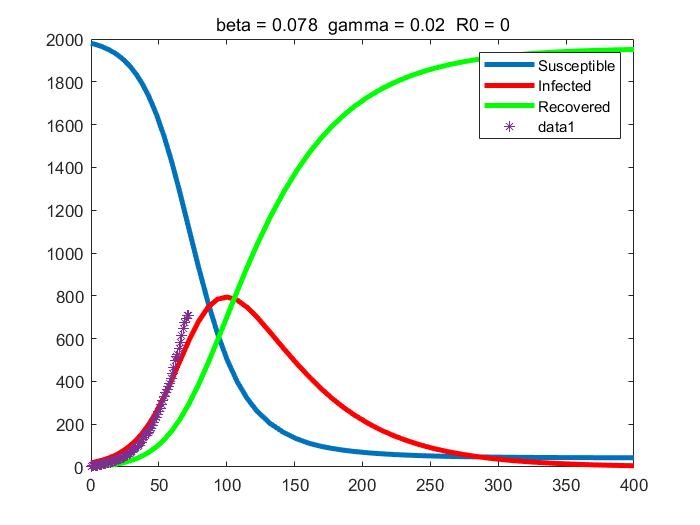
\includegraphics[width=4in]{para1.png}
\caption{parameter set 1}
\end{figure}
\begin{figure}[h]
\centering
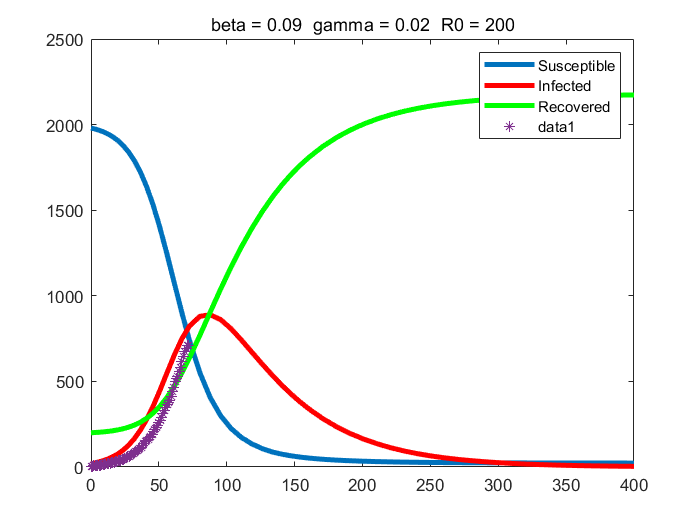
\includegraphics[width=4in]{para2.png}
\caption{parameter set 2}
\end{figure}
\section*{II. Image Denoising and Impainting by PDE}
\begin{figure}[H]
\centering
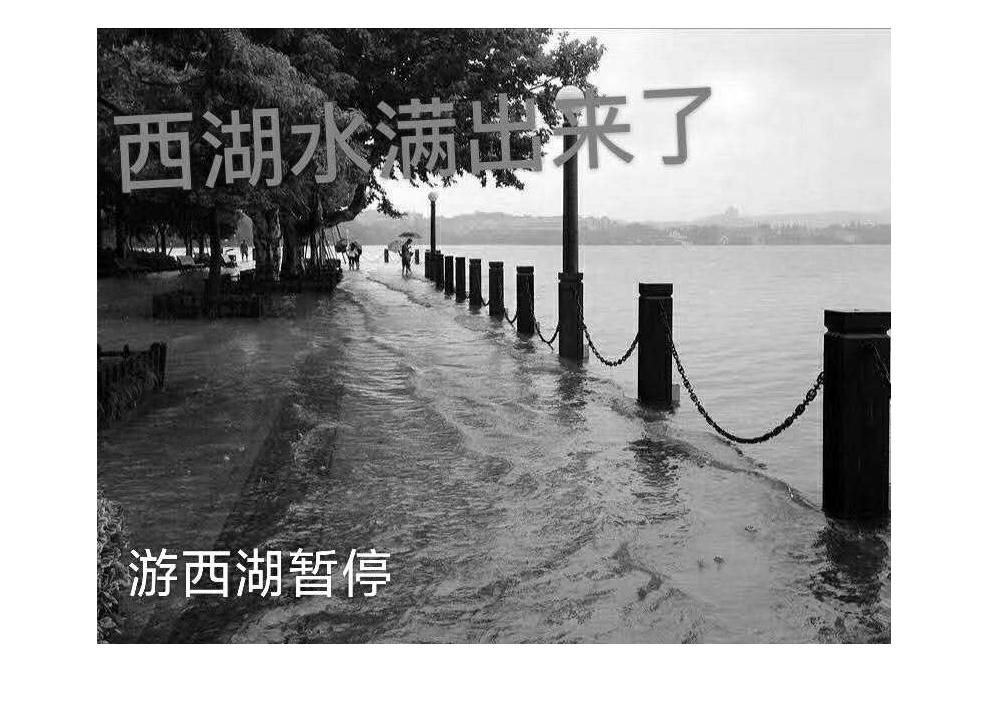
\includegraphics[width=5in]{og.jpg}
\caption{original picture}
\end{figure}
\begin{figure}[H]
\centering
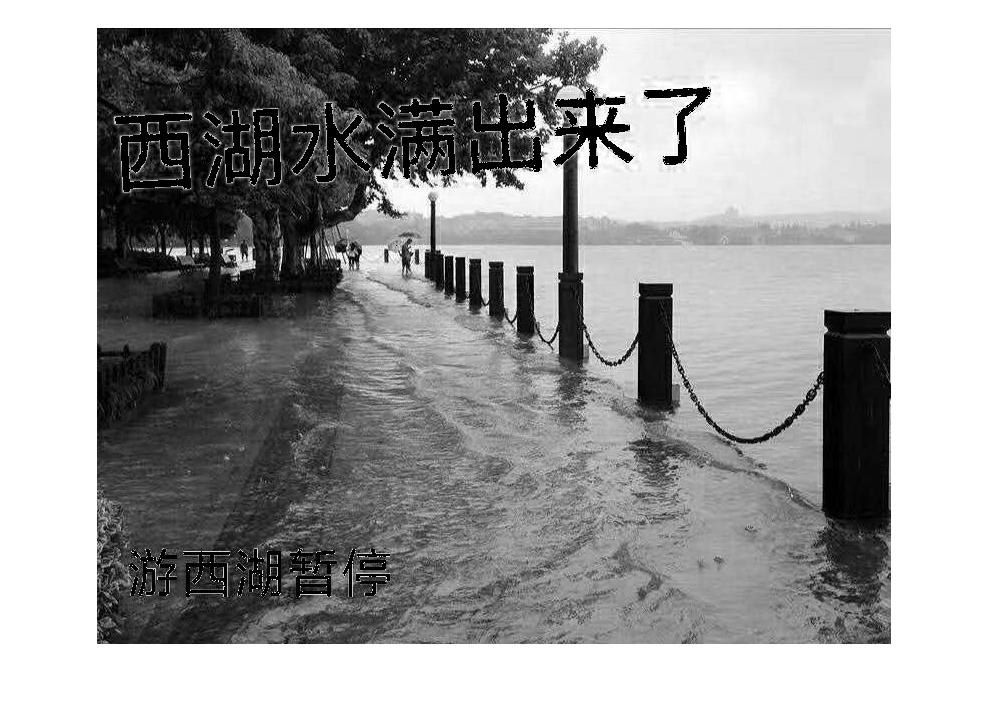
\includegraphics[width=5in]{marked.jpg}
\caption{after marked characters}
\end{figure}
\begin{figure}[H]
\centering
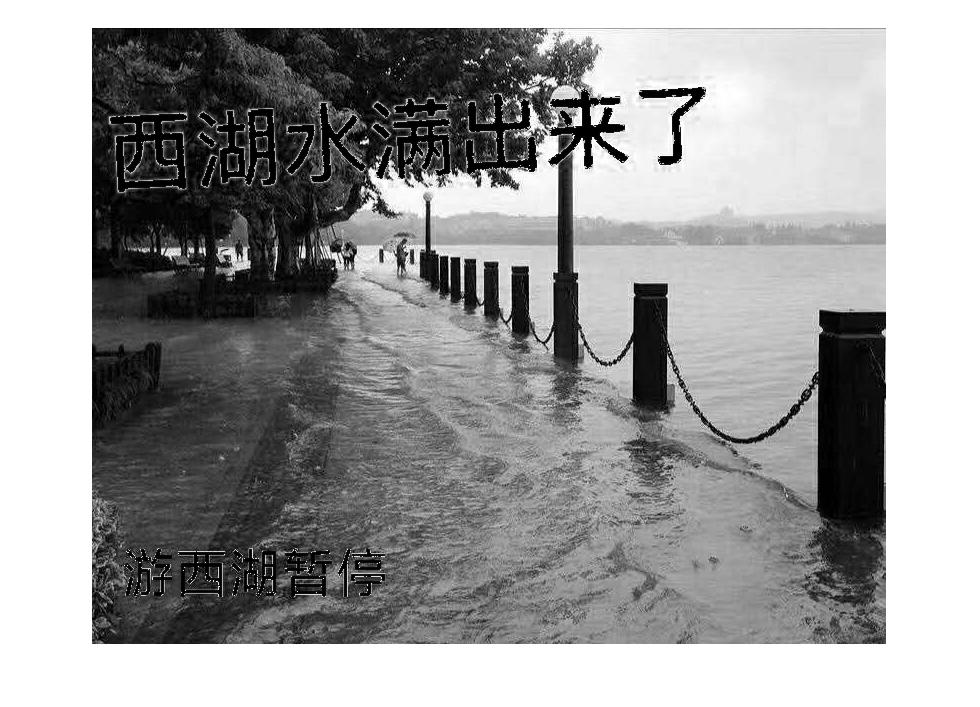
\includegraphics[width=6in]{result.jpg}
\caption{final result}
\end{figure}
Personally, I think this method doesn't work at in this pictureall even though I have iterated for 2000 times.
\end{document}

%%% Local Variables: 
%%% mode: latex
%%% TeX-master: t
%%% End: 
